\section{Internet, IVV~NWZ, Computer\-Labs~\&~Co.}
\begin{multicols*}{2}
	\fibelimgtext[below left]{
		\includegraphics[width=\columnwidth]{private/res/comics/hacker.pdf}
	}{Jan Tomaschoff\qquad© Cartoon-Caricature-Contors, Pfaffenhofen}
\subsection{WLAN für alle!}
Wo mittlerweile viele Restaurants und Cafés freien Internetzugang über WLAN zur Verfügung stellen und Politiker damit werben, das an Münsteraner Schulen fortzuführen, in einer Zeit in der wissenschaftliches Arbeiten ohne den schnellen Austausch relativ großer Daten nicht mehr denkbar ist, gibt es natürlich auch an der Universität eures Vertrauens frei verfügbaren WLAN-Zugang für jeden. Solange er Mitarbeiter oder Student der WWU oder einer am eduroam-Projekt teilnehmenden Hochschule ist.
Außerdem bekommt ihr noch ein ganzes Paket an Cloud-Speichern und könnt im Uni-Netz sogar von überall aus drucken oder eigentlich teure Bücher und Programme herunterladen.

\subsubsection{Und wie funktioniert das?}
Anstatt wie früher zunächst einen Nutzerantrag des Zentrums für Informationsverarbeitung~(ZIV) ausfüllen zu müssen, erhaltet ihr heute bereits mit eurer Einschreibung in die Uni eine Nutzerkennung der Form \texttt{v\_nnnn\#\#} mit zugehörigem Passwort, die aus eurem Vor- und Nachnamen sowie zwei Zahlen gebildet wird -- für "Max Mustermann" wäre eine mögliche Kennung "\texttt{m\_must08}".
Zusätzlich erhaltet ihr eine Uni-E-Mail-Adresse -- hängt für diese einfach \texttt{@uni-muenster.de} oder \texttt{@wwu.de} (funktioniert beides) an eure Nutzerkennung an.

Nutzerkennungen der Uni werden zudem verschiedenen Nutzergruppen zugewiesen; für Studierende der Physik sind das zunächst \texttt{u0dawin} (Studierende) und \texttt{p0stud} (Angehörige der Physik).
So werden bspw.\ Angebote auf Studierende bestimmter Fachbereiche beschränkt.
Allgemein müsst ihr euch aber nicht mit Nutzergruppen auskennen -- das ist eher Detailwissen und passiert im Wesentlichen im Hintergrund.

Was für euch aber wichtig ist, ist, dass ihr, wenn ihr Physik an der WWU studiert, eine ganze Reihe an kostenlosen oder kostengünstigen Angeboten bekommt.

\subsection{Was kann man denn nun alles machen?}
Der wichtigste Dienst ist sicherlich euer E-Mail-Postfach.
Auch wenn ihr vielleicht schon eines oder mehrere davon habt, ist das E-Mail-Postfach der Uni besonders wichtig für euch.
Viele relevanten Infos werden euch darüber geschickt -- So zum Beispiel die Aufforderung, den Semesterbeitrag zu zahlen, oder die Information, dass eine Vorlesung kurzfristig ausfällt.
Ihr seid sogar verpflichtet, die Mails der Universität zu lesen -- Wenn ihr also den Semesterbeitrag nicht zahlt, werdet ihr sogar exmatrikuliert -- also passt auf! Auch die Erinnerung zur Prüfungsanmeldung und unsere Infomails (mit denen wir uns aber sehr zurückhalten, wir wollen euch ja nicht "zuspammen", und auch wir kennen das Problem überfluteter Postfächer :) ) erhaltet ihr per Mail.

Uns, die Fachschaft eures Vertrauens, erreicht ihr übrigens über die Adresse \email{fsphys@uni-muenster.de}.

\subsubsection{Portale}
Im Portal myWWU (\url{https://www.uni-muenster.de/mywwu}) sind die wichtigsten Dienste der Uni zusammengefasst.
Dazu gehören das E-Mail-Postfach, das Vorlesungsverzeichnis (HIS~LSF), ein Kalender (der euch auch erinnert, wann ihr Bücher zurückgeben müsst), von euch ausgewähle Newsfeeds\dots Wenn man MyWWU richtig nutzt, kann es sehr praktisch sein.

Auch sehr nützlich ist der Zugriff auf den OPAC, ein integriertes Katalog- und Ausleihsystem der ULB, und disco (\url{https://disco.uni-muenster.de}), das Suchsystem der ULB.
Hier sind der OPAC und viele weitere Verzeichnisse integriert, sodass ihr in vielen Millionen Dokumenten suchen könnt.
Ihr braucht also nicht jedes Mal zur ULB zu laufen, um Bücher zu verlängern.
Wesentlich wichtiger sind jedoch Buch- und Literaturrecherchen, die ihr schnell und effektiv per Netz an den verschiedensten Stellen machen könnt.
Daneben gibt es über die ULB und den Fachbereich Physik auch einen kostenlosen Zugang zu allen wesentlichen wissenschaftlichen Zeitschriften und zu vielen Bücher z.\,B.\ von Springer.

Ruft dazu aus dem Uni-Netz (oder von zu Hause aus über VPN) die Webseite \url{https://link.springer.com} auf und ladet das Buch eurer Wahl einfach herunter.

\begin{center}
	\includegraphics[width=\columnwidth, height=0.3\textheight]{private/res/comics/computersuechtig.pdf}
\end{center}

\subsubsection[Sichere Datencloud -- sciebo!]{Sichere Datencloud -- sciebo! \cref{internet:sciebo}}
Seit Kurzem bietet die WWU gemeinsam mit anderen nordrhein-westfälischen Hochschulen eine Dropbox-ähnliche Cloud an, die im Gegensatz zu anderen bekannten Online-Speicherdiensten betont nicht-kommerziell ist und viel Wert auf Datenschutz legt.
Ganz abgesehen davon, dass die Idee zur Cloud von einem Fachschaftler kam -- Danke, Markus :) -- ist Sciebo auch wegen seiner guten Umsetzung und einfacher Bedienoberfläche unbedingt empfehlenswert.
Einfach auf \url{https://www.sciebo.de} registrieren und dann mit \texttt{<nutzerkennung>@uni-muenster.de} als Benutzername und dem soeben gewählten Passwort anmelden.
Insgesamt bekommt man dort \SI{30}{\giga\byte} freien Speicherplatz.

\subsubsection{Spielregeln}
Neben reiner Textinformation habt ihr natürlich einen ungefilterten Zugang zum Internet und damit Zugriff auf alle anderen Angebote.
An dieser Stelle eine Warnung, damit es keine bösen Überraschungen gibt: Auch wenn der Zugang zum Internet über das Uninetz recht schnell ist und es viele Mitglieder an der Uni gibt, so können Urheberrechtsverstöße und andere illegale Aktivitäten zu euch zurückverfolgt werden.
Ebenfalls führt der Versand von Spam und Viren z.\,B.\ zu einer Sperrung des Netzzugangs -- So sind die Sanktionen bei Zuwiderhandlung in der Benutzungsordnung geregelt.
Dies soll euch nicht abschrecken, dennoch solltet ihr die Spielregeln kennen.

\subsubsection{ComputerLabs}
An quasi jedem Rechner der WWU habt ihr Zugriff auf euer persönliches Benutzerkonto -- Einfach Nutzerkennung und Passwort eingeben und los geht's.
Der Fachbereich Physik hat, auf mehrere Gebäude verteilt, "ComputerLabs" eingerichtet, an denen eine große Zahl an Rechnern für euch zur Verfügung stehen.
Mit eurer Nutzerkennung könnt ihr übrigens auch die Rechner in den Labs der Biologie und Chemie benutzen -- und umgekehrt.
Dass ihr überall dieselbe Arbeitsumgebung, euer Netzlaufwerk (Laufwerk \texttt{I:} mit \SI{10}{\giga\byte} Speicherplatz) und die gleichen Programme vorfindet, dafür ist gesorgt.
Außerdem gibt es noch allgemein zugängliche ComputerLabs wie die im ZIV~(Einsteinstraße~60).
Diese können von allen Angehörigen der Uni verwendet werden, allerdings stehen euch hier nicht dieselbe Software-Auswahl und Arbeitsumgebung zur Verfügung wie bei den Rechnern des naturwissenschaftlichen Zentrums.
Standardmäßig ist beispielsweise nur euer ZIV-Netzlaufwerk (Laufwerk \texttt{U:} mit \SI{1}{\giga\byte} Speicherplatz) und nicht das \texttt{I}-Laufwerk eingebunden.

Die ComputerLabs der Physik findet ihr an folgenden Orten:
\begin{description}
	\item[Angewandte Physik:] 10~Windows-PCs.
	\item[Institut~für~Kernphysik,] 2.~Stock: 11~Windows-PCs, Scanner, s/w-Laserdrucker.
	\item[Institut~für~Theoretische~Physik,] 4.~Stock: 11 Windows-PCs.
	\item[Institutsgruppe~1~(IG1):]~
		\begin{itemize}[leftmargin=1mm]
			\item StudiBib, Erdgeschoss, Raum~13: Zwei Windows-PCs, Scanner, Farbdrucker.
			\item Institut für Technik und ihre Didaktik (Raum 220): 9~Windows-PCs, s/w-Laserdrucker.
			\item Physikalisches~Institut, 5.~Stock, Räume~504 und 520: insgesamt 9~Windows-PCs, A3-Flachbettscanner, s/w- und Farblaserdrucker.
			\item Institut~für~Festkörpertheorie, Raum~745 und 747: insgesamt 21~Windows-PCs, Scanner, s/w-Laserdrucker.
		\end{itemize}
	\item[Institut~für~Geophysik,] Corrensstr., Raum~301 und 333, je 10~Windows-PCs.
	\item[Seminar für Didaktik des Sachunterrichts]~\\(DDSU) im Leonardo-Campus~11, Raum~104: 9~Windows-PCs, s/w-Laserdrucker.
\end{description}

Die jeweiligen Ansprechpartner bei Fragen, Problemen und auftretenden Fehlern sind im jeweiligen ComputerLab bekanntgegeben.
Auf all diesen Computern ist ein sehr umfangreiches Software-Angebot installiert, sodass ihr dort direkt arbeiten könnt.
Eine Übersicht gibt es auf der Internetseite der IVV~NWZ~\cref{internet:ivvnwz}.

Ein kurzer Hinweis zum Begriff "IVV": Neben dem ZIV, das für die zentrale Bereitstellung von IT an der Uni zuständig ist, gibt es an der Uni zehn  sogenannte dezentrale "Informations-Verarbeitungs-Versorgungseinheiten" (IVV), die für bestimmte Bereiche zuständig sind.
Für die Fachbereiche Biologie, Chemie und Physik ist das die IVV~NWZ (IVV~4).

\fibelimgtext[bottom left]{
	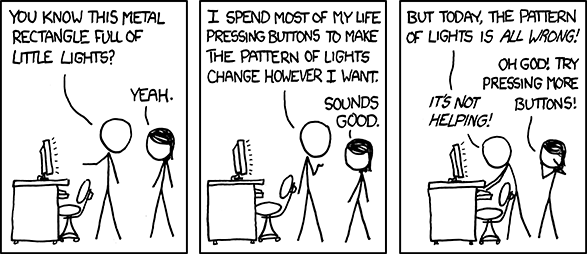
\includegraphics[width=\columnwidth]{res/xkcd/722_computer_problems.png}
}{\url{https://xkcd.com/722}}

\subsubsection[Weitere Angebote der IVV~NWZ und des ZIV]{Weitere Angebote der\\IVV~NWZ und des ZIV}
Sowohl die IVV~NWZ als auch das ZIV betreiben Remote-Desktop-Server, auf die ihr von Zuhause zugreifen könnt.
Damit habt ihr auch von Zuhause aus Zugriff auf die meiste Software und könnt damit arbeiten.
Das Stichwort "Cloud" fällt meist irgendwann in diesem Zusammenhang und sollte heutzutage jedem bekannt sein.
Etwas Ähnliches bieten IVV und ZIV schon seit vielen Jahren allen Studierenden an.
Bei der IVV gibt es \SI{10}{\giga\byte} Speicherplatz (Laufwerk~\texttt{I:}) und beim ZIV \SI{1}{\giga\byte} (Laufwerk~\texttt{U:}), s.~oben.
Dieser Speicherplatz kann auch ähnlich wie eine Festplatte von zuhause angebunden werden.

Auch kostengünstige Druckmöglichkeiten (A4 bis A0, auch in Farbe) werden angeboten; für die Nutzung ist eine kostenlose Anmeldung bei "Print~\&~Pay" (in MeinZIV; Link im Abschnitt~"DPÜ", S.~\pageref{dpü} in dieser Fibel) erforderlich.
Weitere Informationen hierzu und vielen weiteren Angeboten sowie Anleitungen gibt es bei der IVV~NWZ~\cref{internet:ivvnwz} und beim ZIV~\cref{internet:ziv}, sowie in der Ersti-Woche und bei uns~\cref{internet:fsphys_software}.

\subsubsection{Software für Zuhause}
Für Studierende gibt es beim ZIV zwei interessante Softwarepakete, die insbesondere auch für den privaten Einsatz auf den eigenen Computern vorgesehen sind.
Interessant ist vor allem die Anti-Virus-Software (Sophos), welche von der Uni für alle bezahlt wird.
Zusätzlich können viele weitere Programme, die das ZIV betreut, auch auf dem eigenen Rechner installiert und unter einigen Bedingungen genutzt werden~\cref{internet:ziv_software}.

Die IVV~NWZ ermöglicht zudem allen zugehörigen Studierenden den Zugriff auf das Imagine-Programm von Microsoft.
Damit habt ihr Zugriff auf fast die gesamte Software-Palette von Microsoft, nur einige Office-Programme (Word, Excel, PowerPoint) dürfen nicht angeboten werden.
Diese Software dürft ihr ausdrücklich auch auf privaten Rechner installieren.
Weitere Programme wie die Mathematik-Software "Mathematica" (vielen vielleicht bereits durch die -- übrigens fürs Studium häufig nützliche -- Webseite WolframAlpha \cref{internet:wolfram_alpha} bekannt) können ebenfalls unter verschiedenen Bedingungen bezogen werden -- Mathematica kann beispielsweise nur im Uni-Netzwerk (d.\,h.\ zum Beispiel von zuhause über eine VPN-Verbindung) genutzt werden.
Weitere Infos findet ihr wieder unter \cref{internet:ivvnwz}, \cref{internet:ziv} und \cref{internet:fsphys_software}.

\subsection{Links}
\begin{flushleft}
	\begin{fibelurl}
		\url{https://www.sciebo.de}
		\label{internet:sciebo}
	\end{fibelurl}
	\begin{fibelurl}
		\url{https://www.uni-muenster.de/NWZ}
		\label{internet:ivvnwz}
	\end{fibelurl}
	\begin{fibelurl}
		\url{https://www.uni-muenster.de/ZIV}
		\label{internet:ziv}
	\end{fibelurl}
	\begin{fibelurl}
		\url{https://www.uni-muenster.de/Physik.FSPHYS/service/software}
		\label{internet:fsphys_software}
	\end{fibelurl}
	\begin{fibelurl}
		\url{https://www.uni-muenster.de/ZIV/Software/Uebersicht.html}
		\label{internet:ziv_software}
	\end{fibelurl}
	\begin{fibelurl}
		\url{https://www.wolframalpha.com}
		\label{internet:wolfram_alpha}
	\end{fibelurl}
\end{flushleft}

\fibelsig{Simon, Benedikt}

\medskip

\begin{center}
	\fibelimgtext[below right]{
		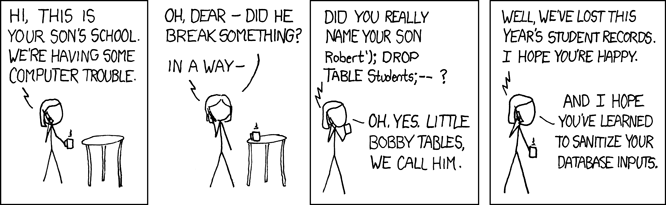
\includegraphics[width=\columnwidth, height=0.2\textheight]{res/xkcd/327_exploits_of_a_mom.png}
	}{\url{https://xkcd.com/327}}
\end{center}
\end{multicols*}

